\documentclass[sigconf]{acmart}
\AtBeginDocument{%
    \providecommand\BibTeX{{%
        Bib\TeX}}}
\acmConference[Konferenz '25]{Konferenz 25, Januar 2025}{Januar 2025}{Hof, Deutschland}
\copyrightyear{2025}
\acmYear{2025}
\acmDOI{1337.69420}

\acmJournal{JACM}
\acmVolume{37}
\acmNumber{4}
\acmArticle{420}
\acmMonth{1}

\renewcommand{\keywordsname}{Schlüsselwörter}
\setcopyright{none}
\thanks{Erlaubnis zur Herstellung digitaler oder gedruckter Kopien dieses Werks, ganz oder teilweise, für den persönlichen oder Unterrichtsgebrauch wird ohne Gebühr erteilt, vorausgesetzt, dass Kopien nicht zum Profit oder kommerziellen Vorteil hergestellt oder verbreitet werden und dass Kopien diesen Hinweis sowie die vollständige Zitierung auf der ersten Seite tragen. Urheberrechte für Bestandteile dieses Werks, die nicht den Autor(en) gehören, müssen beachtet werden. Das Abstraktieren mit Angabe der Quelle ist gestattet. Für anderweitige Vervielfältigung, Veröffentlichung, das Posten auf Servern oder das Weiterverbreiten in Listen ist eine vorherige spezifische Erlaubnis und/oder Gebühr erforderlich. Erlaubnisse können bei sebastian.peschke@proton.me angefragt werden. Konferenz ’25, Januar 2025, Hof, Deutschland. © 2025 Urheberrecht liegt beim Eigentümer/Autor(en). Veröffentlichungsrechte lizenziert an Hochschule Hof. ISBN 978-x-xxxx-xxxx-x/YY/MM... \$15.00. https://doi.org/1337.69420}
\usepackage{listings}
\usepackage{tikz}
\usepackage{csquotes}
\usepackage{glossaries}
\usetikzlibrary{shapes.geometric, arrows}
\renewcommand{\figurename}{Abbildung}
\usepackage[ngerman]{babel}
\usepackage{siunitx}

\begin{document}
    \thispagestyle{firstpagestyle}
    %! Author = charon
%! Date = 11/21/24
\title{Fuzzing}
\subtitle{Ein umfassender Überblick und Machine Learning Ansätze}
\author{Sebastian Peschke}
\authornote{}
\email{sebastian.peschke@hof-university.de}
\orcid{1234-5678-9012}
\authornotemark[1]
\affiliation{
    \institution{Institut für Informationssysteme Hof}
    \city{Hof}
    \state{Bayern}
    \country{Germany}
}
\renewcommand{\shortauthors}{Peschke}

    %! Author = charon
%! Date = 11/20/24
\begin{abstract}
    A clear and well-documented \LaTeX\ document is presented as an
    article formatted for publication by ACM in a conference proceedings
    or journal publication. Based on the ``acmart'' document class, this
    article presents and explains many of the common variations, as well
    as many of the formatting elements an author may use in the
    preparation of the documentation of their work.
\end{abstract}
    \keywords{Fuzzing, Testing, Automation, Security, Machin Learning, Reverse Engineering, Network Security, Binary Analysis,
      Vulnerability Detection, Exploit Generation, Program Analysis, Program Optimization}
    \maketitle
    %! Author = charon
%! Date = 11/20/24

\section{Einführung}\label{sec:introduction}
Fuzzing ist eine Technik zur Identifikation von Sicherheitslücken und Programmfehlern in Software.
Durch die automatisierte Generierung und Überprüfung von Eingabedaten werden Schwachstellen identifiziert.
Im Kern basiert Fuzzing auf der systematischen oder zufälligen Erzeugung von Testdaten, die an das System unter Test (SUT) übermittelt
werden, um dessen Verhalten unter außergewöhnlichen Bedingungen zu analysieren.
Die Ergebnisse werden genutzt, um Abstürze, Speicherfehler oder andere unerwünschte Zustände zu detektieren.\newline
Die Integration von Künstlicher Intelligenz (KI) und Machine Learning (ML) in das Fuzzing kann zur Verbesserung der
Effizienz und Effektivität durch Automatisierung von Entscheidungsprozessen und Optimierung der Testdatengenerierung führen.
LLMs wie GPT oder BERT~\cite{devlin_bert_2019} haben sich als leistungsfähig bei der Analyse und Generierung von natürlicher Sprache und
strukturierten Daten erwiesen.\newline
Im Kontext von Fuzzing können LLMs genutzt werden, um semantisch sinnvolle Testeingaben für Anwendungen zu generieren,
die stark strukturierte oder grammatikabhängige Eingaben erwarten~\citet{deng_large_2023}.
Durch ihre Fähigkeit syntaktische und semantische Abhängigkeiten in komplexen Eingabeformaten zu verstehen können LLMs helfen
die Effizienz des Fuzzing-Prozesses zu steigern.\newline
Auch Generative Adversarial Networks (GAN) können im Fuzzing eingesetzt werden, um realistische Testeingaben zu generieren.
GANs bestehen aus einem Generator- und einem Diskriminator-Modell.
Im Fuzzing-Umfeld können sie eingesetzt werden, um Eingabedaten zu erzeugen, die spezifische Eigenschaften oder Schwachstellen
adressieren.
Beispielsweise könnte der Generator synthetische Testfälle erzeugen, die mögliche Schwachstellen in der Eingabeverarbeitung
eines Programms explorieren, während der Diskriminator -- in diesem Kontext das SUT mit Monitoring-Mechanismen -- die Qualität
der erzeugten Eingaben bewertet~\citet{devlin_bert_2019}.
Dies erlaubt die Generierung diverser und relevanter Testfälle, insbesondere für Programme mit komplexen Anforderungen.\newline
Im Kontext des Fuzzings kann Reinforcement Learning (RL) genutzt werden, um die Sequenz von Eingaben oder Teststrategien zu optimieren.
Hierbei wird ein Agent trainiert, der durch Interaktionen mit dem Zielprogramm lernt, Eingaben zu generieren, die mit
höherer Wahrscheinlichkeit Schwachstellen auslösen.
Belohnungsfunktionen können beispielsweise auf Metriken wie Codeabdeckung, Anomalien im Speicherzugriff oder spezifischen
Abstürzen basieren~\cite{paduraru_riverfuzzrl_2021}.\newline
Die Kombination von Fuzzing-Methoden mit KI-gestützten Ansätzen bietet Potenziale.
Beispielsweise können durch die Nutzung von LLMs, GANs und RL neue Eingabemuster erschlossen werden, die mit traditionellen Techniken
nur schwer zu herauszufinden.
Existierend Herausforderungen, wie die Skalierbarkeit der Ansätze bei hochkomplexen Programmen, die hohe Rechenintensität von
ML-Modellen sowie die Erklärbarkeit und Vertrauenswürdigkeit der generierten Ergebnisse bleiben dennoch bestehen und
stellen ein weiteres Forschungsproblem in der Zukunft dar~\cite{ramadan_role_2024}.
    %! Author = chaorn
%! Date = 17.01.25

\section{Verwandte Arbeiten}\label{sec:related-work}
Zu dem Thema Anwendungsgebiete für ML-Techniken in Fuzzing gibt es bereits einige Arbeiten, die sich mit der Thematik auseinandersetzen.
\citet{saavedra_review_2019} untersuchen die Integration von ML in Fuzzing-Prozesse und heben dabei die Anwendungen in der
Eingabegenerierung und der Post-Fuzzing-Analyse hervor.
Gleichzeitig identifizieren sie Herausforderungen wie Datenbeschränkungen und die rechnerische Komplexität.\newline
\citet{wang_systematic_2020} liefern eine systematische Übersicht über den Einsatz von ML-Techniken im Fuzzing.
Sie diskutieren verschiedene Phasen, in denen ML angewendet werden kann, die verwendeten Algorithmustypen sowie die
Leistungsmetriken zur Bewertung dieser Methoden.\newline
\citet{zhong_neural_2022} stellen mit AutoFuzz einen grammatikgesteuerten Ansatz für das Fuzzing von autonomen Fahrzeugen
vor, der auf ML basiert.
AutoFuzz kombiniert evolutionäre Algorithmen mit neuronalen Netzen, um komplexe Fahrszenarien in Simulationen zu generieren,
die zu vielfältigen Verkehrsverstößen führen können.
Die Ergebnisse zeigen, dass AutoFuzz im Vergleich zu Baseline-Methoden \num{10}\text{--}\num{39}\,\unit{\percent}
mehr einzigartige Verkehrsverstöße entdeckt und somit die Robustheit von AV-Software verbessern kann.\newline
\citet{she_mtfuzz_2020} führen mit MTFuzz ein neuartiges Fuzzing-Framework ein, das auf Multi-Task Neuronalen Netzwerken basiert.
Durch die Nutzung eines kompakten Embeddings und Gradient-basierter Mutationen verbessert MTFuzz die Abdeckung von
Programmverzweigungen.
Es deckt bis zu dreimal mehr Kanten ab als aktuelle state-of-the-art Fuzzer und identifiziert dabei elf zuvor unbekannte
Softwarefehler.\newline
\citet{chen_learning-guided_2019} entwickeln eine ML-gestützte Fuzzing-Technik für Cyber-Physical Systems (CPS), die intelligente
Angriffe auf Netzwerke von Aktoren simuliert, um unsichere physische Zustände zu erzeugen.
Mithilfe eines prädiktiven Modells und heuristischer Suche generiert diese Methode Testfälle, die spezifische
Sicherheitsmechanismen von CPS prüfen.
In zwei realen CPS-Testbeds identifizierte der Ansatz 27 unsichere Zustände, darunter sechs, die in etablierten Benchmarks
nicht enthalten waren.
    %! Author = charon
%! Date = 11/21/24

\section{Hintergrund}\label{sec:hintergrund}
Das Fuzzing besteht aus mehreren Komponenten und Herangehensweisen.
Diese Methodiken und Strategien sind entscheidend für die Effektivität des Fuzzings und die
Identifizierung von Schwachstellen.
Im Folgenden werden die wesentlichen und Bereiche des Fuzzings erläutert und die Limitationen des Fuzzings aufgezeigt.
\subsection{Fuzzing Herangehensweisen}\label{subsec:testing-methoden}
Es gibt drei grundlegende Herangehensweisen an das Fuzzing: Black Box, White Box und Grey Box Fuzzing.
\begin{itemize}
    \item Black Box Fuzzing
    \item White Box Fuzzing
    \item Grey Box Fuzzing
\end{itemize}
\subsection{Sparten des Fuzzing}\label{subsec:sparten-des-fuzzing}
\begin{enumerate}
    \item \textit{IoT Fuzzing}: Das Fuzzing im Internet der Dinge (IoT) konzentriert sich auf die Sicherheitsprüfung von IoT-Geräten, die aufgrund ihrer
    spezifischen Merkmale und ressourcenbedingten Einschränkungen häufig anfällig sind.
    Die Sicherheitsherausforderungen im IoT unterscheiden sich signifikant von denen traditioneller IT-Systeme, da IoT-Geräte
    oftmals über keine ausreichenden Sicherheitsmechanismen verfügen~\cite{eceiza_fuzzing_2021}.
    \item \textit{Firmware-Fuzzing}: Firmware-Fuzzing zielt auf die Firmware von Geräten ab, die als Low-Level-Software die Hardware-Komponenten steuert.
    Diese Methode ist besonders wichtig, da Firmware oft Schwachstellen enthält, die von Angreifern ausgenutzt werden können.
    Die Effektivität des Fuzzings in diesem Kontext hängt von der Fähigkeit ab, Eingaben zu generieren, die mit den Funktionen
    der Firmware interagieren.
    Zu den Herausforderungen zählen die notwendige Kenntnis der Firmware-Struktur sowie ressourcenbedingte Einschränkungen,
    die den Fuzzing-Prozess limitieren können~\cite{eceiza_fuzzing_2021}.
    \item \textit{Binary-Fuzzing}: Binary-Fuzzing konzentriert sich auf die Analyse von kompilierten Binärdateien anstelle von Quellcode.
    Diese Technik ist insbesondere für proprietäre Software ohne zugänglichen Quellcode von Bedeutung.
    Hierbei werden zufällige oder semi-zufällige Eingaben an die Binärdateien übermittelt, um Abstürze oder unerwartetes Verhalten
    zu detektieren.
    Die Herausforderung besteht in der fehlenden Transparenz über die interne Funktionsweise der Binärdateien, was die Erstellung
    effektiver Testfälle erschwert.
    Dennoch können durch Binary-Fuzzing kritische Schwachstellen aufgedeckt werden, die mit anderen Testmethoden möglicherweise
    unentdeckt bleiben~\cite{eceiza_fuzzing_2021}.
    \item \textit{Netzwerkprotokoll-Fuzzing}: Das Netzwerkprotokoll-Fuzzing dient der Prüfung der Robustheit von Netzwerkprotokollen, indem fehlerhafte oder unerwartete
    Pakete an einen Netzwerkdienst gesendet werden.
    Diese Art des Fuzzings ist entscheidend, um Schwachstellen in Kommunikationsprotokollen zu identifizieren, die von
    Angreifern ausgenutzt werden könnten, um unbefugten Zugriff zu erlangen oder Dienste zu stören.
    Für die effektive Generierung von Testfällen ist ein Verständnis der Protokollspezifikationen unerlässlich, wie die Arbeit
    betont~\cite{eceiza_fuzzing_2021}.
    \item \textit{Betriebssystem-Fuzzing}: Das Betriebssystem-Fuzzing befasst sich mit der Sicherheitsprüfung des Betriebssystems selbst, um Schwachstellen zu identifizieren,
    die von Schadsoftware oder böswilligen Nutzern ausgenutzt werden könnten.
    Diese Technik ist von zentraler Bedeutung, da Sicherheitslücken auf Betriebssystemebene schwerwiegende Konsequenzen wie
    unbefugten Zugriff oder Datenverluste nach sich ziehen können.
    Zu den Herausforderungen zählen die hohe Komplexität der Betriebssystemarchitektur sowie die Notwendigkeit, eine umfassende
    Abdeckung der verschiedenen Systemkomponenten zu gewährleisten~\cite{eceiza_fuzzing_2021}.
\end{enumerate}
\subsection{Limitationen des Fuzzing}\label{subsec:limitationen-des-fuzzign}
Fuzzing hat einige Limitationen, die seine Effektivität einschränken können:\newline
\textit{Lückenhafte Codeabdeckung}:
Komplexe Programme mit tief verschachtelten Bedingungen oder umfangreichen Verzweigungen können dazu führen, dass bestimmte
Codepfade ungetestet bleiben.
Dies resultiert aus der Schwierigkeit, Eingaben zu generieren, die alle möglichen Pfade durchlaufen.
Zudem können Techniken wie Code-Obfuskation die Effektivität von Fuzzern beeinträchtigen, indem sie die Pfadanzahl
künstlich erhöhen und somit die Analyse erschweren~\cite{wachter_fuzzing}.\newline
\textit{Unzureichende Testfälle}:
Die Qualität der durch Fuzzing generierten Testfälle hängt von der eingesetzten Strategie ab.
Black-box-Fuzzing kann ineffizient sein und wichtige Fehler übersehen.
Obwohl Gray-box-Fuzzing durch Instrumentierung versucht, ein Gleichgewicht zu finden, bleibt die Herausforderung
bestehen, für alle Szenarien -- vor allem bei umfangreichen Systemen -- zureichende Testfälle zu generieren.\newline
\textit{Verstehen von komplexen Codepfaden}:
Komplexe Codepfade, insbesondere solche mit tiefen Verschachtelungen oder zahlreichen Bedingungen, stellen für Fuzzer eine
Herausforderung dar.
Die Pfadexplosion, also die exponentielle Zunahme möglicher Pfade, kann dazu führen, dass nicht alle relevanten Pfade
effektiv getestet werden.
Obwohl hybride Ansätze, die Fuzzing mit symbolischer Ausführung kombinieren, entwickelt wurden, um diese Hürde zu beheben,
bleibt die vollständige Abdeckung komplexer Pfade eine Herausforderung~\cite{noller_badger_2018}.\newline
\textit{Nichtdeterministische Programme und zustandsabhängige Systeme}:
Programme, deren Verhalten von internen Zuständen oder externen Faktoren abhängt, erschweren die Anwendung von Fuzzing.
Nichtdeterministisches Verhalten kann dazu führen, dass identische Eingaben unterschiedliche Ergebnisse produzieren, was
die Reproduzierbarkeit von Tests beeinträchtigt.
Zudem können zustandsabhängige Systeme, die auf spezifischen Sequenzen von Eingaben reagieren, von traditionellen
Fuzzing-Ansätzen nur unzureichend getestet werden.
Obwohl fortschrittliche Fuzzer versuchen, Zustandsinformationen zu integrieren, bleibt die effektive Handhabung
nichtdeterministischer und zustandsabhängiger Systeme eine offene Forschungsfrage~\cite{she_fox_2024,pham_aflnet_2020}.


    %! Author = charon
%! Date = 11/21/24

\section{Unterscheidung von Fuzzing-Ansätzen}\label{sec:unterscheidung-von-fuzzern}
\subsection{Input Generation}\label{subsec:input-generation}

\subsection{Intelligenz des Fuzzers}\label{subsec:intelligenz-des-fuzzers}

\subsection{Explorationsstrategien}\label{subsec:explorationsstrategien}

    %! Author = charon
%! Date = 11/21/24
\section{Funktionsweise von Fuzzern}\label{sec:funktionsweise}
Die Funktionsweise eines Fuzzers kann im Wesentlichen fünf Komponenten (sieheAbb.~\ref{fig:struktur_fuzzing}) zugeordnet werden:
\begin{itemize}
    \item \textbf{Initialisierung:} Der Fuzzer wird mit einer Menge von Testcases -- auch \textit{Corpus} genannt -- initialisiert, die an das SUT übergeben werden.
    \item \textbf{Dry Run:} Die Testcases werden an das SUT übergeben, um zu überprüfen, ob das SUT durch die Eingaben zum
        Absturz gebracht werden kann.
    \item \textbf{Mutator:} Der Mutator ist für die Generierung neuer Testcases verantwortlich.
    \item \textbf{Feedback:} Das Feedback des SUT wird verwendet, um die Testcases zu verfeinern.
    \item \textbf{System unter Test:} Stellt das zu testende Programm dar.
\end{itemize}
Im Fall von AFL können diese Komponenten etwas feingranularer betrachtet werden.
Der Corpus wird in zwei Teile unterteilt: \textit{Queue} und \textit{Dictionary}~\cite{afl_whitepaper}.
Die Queue enthält die Testcases, die noch nicht an das SUT übergeben wurden.
Sie wird anhand der Feedbackinformationen des SUT priorisiert.
Im Fall von AFL wird die Queue nach der \textit{Coverage} sortiert.
Das Dictionary enthält Tokens, Strings oder Schlüsselwörter, die in den Testcases enthalten sind.
Der Mutator verwendet bei der Generierung neuer Testcases die Informationen aus dem Dictionary, um die Wahrscheinlichkeit
zu erhöhen, einen validen Testcase mittels Mutation zu generieren.
Ein Anwendungsbeispiel für das Dictionary ist eine Sammlung von protokollspezifischen Begriffen wie \texttt{GET} oder
\texttt{POST} bei der Überprüfung von HTTP-Implementierungen.~\newline
Hinzu kommt ein Mutator für die Generierung neuer Testcases.
Dieser Mutator verwendet verschiedene Mutationstechniken, um die Testcases zu verfeinern.
Dazu gehören beispielsweise \textit{Bitflips}, \textit{Byteflips}, \textit{Arithmetische Operationen} oder
\textit{Splicing}~\cite{afl_whitepaper}.\newline
Um das Fuzzing Architektur unabhängig zu gestalten, wird unter AFL die Laufzeitumgebung \texttt{QEMU} verwendet.
Sie ermöglicht es, das SUT in einer virtuellen Umgebung auszuführen, um die Auswirkungen von Abstürzen zu minimieren.
Außerdem wird die Laufzeitumgebung genutzt, um die Testcases zu instrumentieren und das Feedback des SUT zu sammeln.
Hierzu wird das SUT in einem \textit{Forkserver}~\cite{afl_whitepaper} gestartet, der die Testcases an das SUT übergibt und das Feedback
zurückgibt.
Zu beachten ist hierbei, dass für einen Durchlauf des Fuzzers ein neuer Prozess gestartet wird, welcher das SUT ausführt,
die Eingabe an das SUT übergibt und anschließend das SUT -- insofern kein Absturz des SUT provoziert wurde -- kontorlliert
terminiert.
Falls das SUT jedoch mit der Architektur des Host-Systems übereinstimmt, kann das SUT direkt auf dem Host-System ausgeführt
werden, um unnötigen Overhead zu vermeiden und den Fuzzing-Prozess zu beschleunigen.\newline
AFL bietet zudem die Möglichkeit mehrere Strategien für den Ablauf einer Fuzzing-Kampagne zu bestimmen.
Dazu gehören \textit{Code Coverage}, \textit{Black-box Fuzzing} bei der keine Feedbackinformationen verwendet werden und
der \textit{persistent mode}, bei dem der Fuzzer persistent und nicht nach jedem Testcase neu gestartet wird.
Der persistent mode beinhaltet ebenfalls die Funktion einen Adressbereich im Adressraum des SUT zu definieren, in dem der
Fuzzer die Testcases ausführt.
Das kann zu einem erheblichen Performancegewinn führen, da der Fuzzer nicht nach jedem Testcase neu gestartet werden muss
und zeitintensive Berechnungen und Calls zu überspringen~\cite{afl_whitepaper}.
\begin{figure}
    \centering
    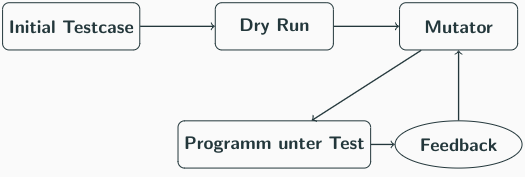
\includegraphics[width=\columnwidth]{res/Struktur_eines_fuzzing_prozesses}
    \caption[Struktur eines Fuzzing Prozesses]{
        Diese Abbildung zeigt den Ablauf eines Fuzzing Prozesses am Beispiel des Fuzzers AFL.
        Der Fuzzer verwendet die bereits gesammelten Testcases.
        Sie werden an das SUT in einer \enquote{Dry Run}-Phase übergeben, um zu überprüfen, ob es durch diese Eingaben
        bereits zum Absturz gebracht werden kann.
        Das Programm wird mit den Eingaben ausgeführt und die Ausgabe wird analysiert.
        Anhand der Analyseergebnisse wird ein Mutator verwendet, um neue Testcases zu generieren, die anhand der initial
        übergebenen Eingaben besonders tief in das Programm eingedrungen sind.
        Die vom Mutator generierten Eingaben werden an das SUT übergeben und das erlangte Feedback des SUT wird zur weiteren
        Verfeinerung der Eingaben verwendet.
        Somit bildet sich ein iterativer Prozess, der die Testcases immer weiter verfeinert.
    }\label{fig:struktur_fuzzing}
\end{figure}

    %! Author = charon
%! Date = 11/21/24
\section{Strategien zur Generation von Eingabedaten}\label{sec:strategien-von-fuzzern-zur-eingabegenerierung}
\begin{figure*}[ht]
    \centering
    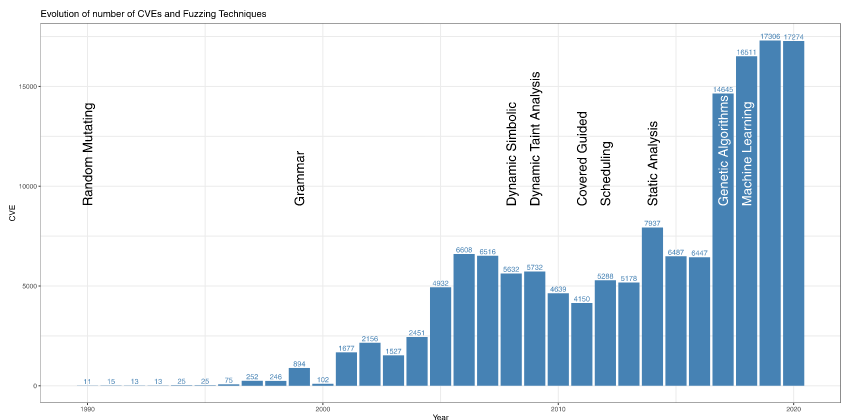
\includegraphics[width=\textwidth]{res/entwicklung_der_eingabestrategien}
    \caption{Eine Übersicht der Entwicklung von Eingabestrategien und deren Einfluss auf die Anzahl der neu aufgedeckten Schwachstellen
    über Zeit.
    Diese Abbildung wurde dem Paper von ~\citet{eceiza_fuzzing_2021} mit einverständnis nach der Creative Commons Attribution 4.0 Lizenz entnommen.}
    \label{fig:eingabestrategien}
\end{figure*}
Die Generierung von Eingabedaten ist ein zentraler Bestandteil des Fuzzings.
Die Qualität und Vielfalt der generierten Eingaben beeinflussen die Effektivität des Fuzzings.
Direkt verbunden mit der Entwicklung von Eingabegenerationsstrategien sind die Anzahl der neu aufgedeckten Schwachstellen (siehe Abb.\ ~\ref{fig:eingabestrategien}).
\subsection{Zufällige Mutation}\label{subsec:zufallige-mutation}
Die Random Mutation beinhaltet die Veränderung von Teilen einer Eingabe, um neue Testfälle für das
Fuzzing zu generieren.
Mutationsbasierte Fuzzer treffen dabei zwei entscheidende Entscheidungen: Wo soll die Mutation erfolgen und welchen neuen
Wert soll sie annehmen?
Häufige Techniken umfassen die Zufallsmodifikation von Bits, gezielte Bit-Flip-Operationen und Änderungen an Ganzzahlen.
Allerdings fehlt diesen Fuzzern das Bewusstsein für das erwartete Eingabeformat, was ihre Effektivität einschränken kann~\cite{saavedra_review_2019}.
\subsection{Regel- und Grammatikbasierte Mutation}\label{subsec:regelbasierte-muataion-und-grammatik}
Regel- und grammatikbasierte Mutationsansätze nutzen Eingabespezifikationen, um die Generierung neuer Eingaben gezielt
zu steuern.
Die Eingabesperifikationen können in Form von Grammatiken, regulären Ausdrücken oder anderen formalen Sprachen vorliegen,
welche der Anwender des Fuzzers zuvor selbst festlegen muss.
Diese Fuzzer erzielen eine bessere Codeabdeckung im Vergleich zu rein mutationsbasierten Fuzzern, da sie auf dem Wissen
über erwartete Eingabeformate basieren.
Allerdings erfordert die Entwicklung präziser Spezifikationen erheblichen Aufwand, was die Implementierung solcher Techniken
komplexer macht.
Diese Komplexität is besonders unter proprietären Softwarelösungen ohne verfügbaren Quellcode problematisch~\cite{eceiza_fuzzing_2021}.
\subsection{Dynamic Taint Analysis}\label{subsec:dynamic-taint-analysis}
Die Dynamic Taint Analyse verfolgt den Informationsfluss von Eingaben -- welche zur Laufzeit des Programms kontaminiert
werden -- zu sensiblen Operationen.
Sie ermöglicht die Erkennung von Schwachstellen, indem überwacht wird, wie Daten die Programmausführung beeinflussen.
Hierzu werden Speicherbereiche wie bspw.\ Register oder Speicherzellen markiert, um den Informationsfluss zu verfolgen.
Herausforderungen wie Overtainting und Undertainting können jedoch die Genauigkeit der Analyse beeinträchtigen, was zu
Fehlalarmen oder übersehenen Schwachstellen führt.
Overtainting tritt auf, wenn zu viele Daten als kontaminiert markiert werden, obwohl sie nicht kontaminiert wurden und
valide Eingaben darstellen und somit falschen Alarm schlagen.
Undertainting trifft zu, wenn kontaminierte Eingaben nicht als solche markiert werden~\cite{schwartz_all_2010}.
\subsection{Dynamic Symbolic execution}\label{subsec:dynamic-symbolic-execution}
Dynamic Symbolic Execution ermöglicht eine Sicherheitsanalyse, indem die Codeausführung überwacht und logische Formeln
erstellt werden, die die Ausführungspfade beschreiben.
Diese Technik hilft, Schwachstellen zu identifizieren, indem unterschiedliche Programmzustände erkundet werden.
Sie kann mit anderen Techniken wie der dynamischen Taint-Analyse kombiniert werden, um die Effektivität zu steigern.
Hier~\cite{schwartz_all_2010}
\subsection{Guided Covered}\label{subsec:guided-covered}
Techniken zur Guided Coverage nutzen Codepfade, um Strategien zur Eingabegenerierung zu
steuern.
Ziel ist es viele Programmpfade mit möglichst wenigen Eingaben zu traversieren.
Die Programmabdeckung wird dabei mithilfe von Instrumentierungstechniken, wie bspw.\ virtuellen Laufzeitumgebungen oder
Injektion eigener Instruktionen (Flags) in den Programmcode, gemessen~\cite{eceiza_fuzzing_2021}.
\subsection{Scheduling}\label{subsec:scheduling}
Das Input Scheduling ist eine Gray-box technik und kann in zwei phasen unterteilt werden:
\begin{enumerate}
    \item \textit{Explorationsphase}: In dieser Phase wird der Speicher teilweise markiert, um Eingabewerte im Speicher
    zu beobachten, wenn bestimmte Instruktionen, wie Vergleichsoperationen, ausgeführt werden.
    Diese Analyse des Speichers ermöglicht es, Eingabewerte mit Speicherzuständen zu verknüpfen (als Konfiguration bezeichnet)
    und fundierte Vermutungen darüber anzustellen, welche Werte ersetzt werden sollten~\cite{eceiza_fuzzing_2021}.
    \item \textit{Exploitationsphase}: In dieser Phase werden die generierten Eingaben teilweise kontaminiert und anhand des
    Feedbacks des SUT erraten, welche Werte ersetzt werden sollten.
    Die bereits gesammelten Daten werden zum Erraten neuer, potenziell schädlicher Werte verwendet~\cite{eceiza_fuzzing_2021}.
\end{enumerate}
\subsection{Statische Analyse}\label{subsec:statische-analyse}
Die statische Analyse untersucht den Code, ohne ihn auszuführen, und ermöglicht so die Identifikation potenzieller
Schwachstellen und Probleme in der Codequalität.
Diese Technik ergänzt dynamische Analyseansätze, da sie Einblicke in die Code-Struktur und mögliche Schwachstellen bietet,
die während der Ausführung nicht erkennbar sind~\cite{wang_systematic_2020}.
\subsection{Genetische Algorithmen}\label{subsec:genetische-algorithmen}
Diese Technik kann als Black-box-, Gray-box- oder White-box-Ansatz umgesetzt werden.
Sie nutzt ein suchbasiertes Optimierungsverfahren, das nach dem Prinzip der natürlichen Selektion arbeitet, um die
bestmöglichen Lösungen für komplexe Probleme zu finden.
Im Bereich des Fuzzings wird die Suche nach Schwachstellen als Optimierungsproblem betrachtet, wobei jede Kandidatenlösung
(Individuum) eine mögliche Fuzzing-Eingabe darstellt.
Die Tauglichkeit bewertet die Nähe zu einer Schwachstelle im SUT, basierend auf dynamischen und
statischen Informationen, wie z.B.\ strukturelle Komplexität~\cite{eceiza_fuzzing_2021}.

    %! Author = chaorn
%! Date = 17.01.25

\section{Machine Learning in Fuzzing}\label{sec:machine-learning-in-fuzzing}

    %! Author = charon
%! Date = 11/21/24

\section{Konklusion}\label{sec:konklusion}
    \bibliographystyle{ACM-Reference-Format}
    \bibliography{src}
    \appendix
\end{document}
\endinput
